% =====================================================
% 题型：函数与图象单选题 (q_tjw_20260605_04_function_graph.tex)
% =====================================================
% =====================================================
% 难度：★★ (中档)
% =====================================================
\newcommand{\qFunctionGraphStem}{%
  函数 $y=\left(x+\dfrac{1}{x}\right)\sin x$ ($x \in [-\pi, 0) \cup (0, \pi]$) 的图象可能是%
}

\newcommand{\qFunctionGraphOptions}{%
  \mcoptions[2]{
    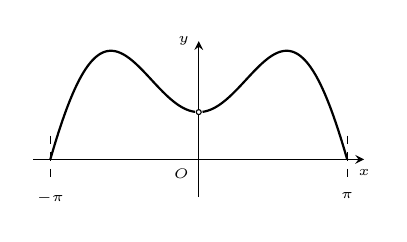
\begin{tikzpicture}[scale=0.6, >=stealth, baseline=(current bounding box.center)]
      \draw[->] (-3.5,0) -- (3.5,0) node[below] {\tiny $x$};
      \draw[->] (0,-0.8) -- (0,2.5) node[left] {\tiny $y$};
      \node[below left] at (0,0) {\tiny $O$};
      \draw[dashed] (3.14,0.5) -- (3.14,-0.5) node[below] {\tiny $\pi$};
      \draw[dashed] (-3.14,0.5) -- (-3.14,-0.5) node[below] {\tiny $-\pi$};
      \draw[thick, domain=0.08:3.14, samples=100] plot (\x, {(\x + 1/\x)*sin(\x r)});
      \draw[thick, domain=-3.14:-0.08, samples=100] plot (\x, {(\x + 1/\x)*sin(\x r)});
      \filldraw[fill=white, draw=black, thin] (0, 1.0) circle (1.5pt);
    \end{tikzpicture}
  }{
    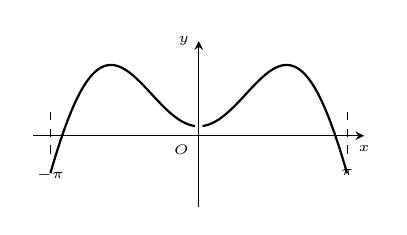
\begin{tikzpicture}[scale=0.6, >=stealth, baseline=(current bounding box.center)]
      \draw[->] (-3.5,0) -- (3.5,0) node[below] {\tiny $x$};
      \draw[->] (0,-1.5) -- (0,2.0) node[left] {\tiny $y$};
      \node[below left] at (0,0) {\tiny $O$};
      \draw[dashed] (3.14,0.5) -- (3.14,-0.5) node[below] {\tiny $\pi$};
      \draw[dashed] (-3.14,0.5) -- (-3.14,-0.5) node[below] {\tiny $-\pi$};
      \draw[thick, domain=0.08:3.14, samples=100] plot (\x, {(\x + 1/\x)*sin(\x r) - 0.8});
      \draw[thick, domain=-3.14:-0.08, samples=100] plot (\x, {(\x + 1/\x)*sin(\x r) - 0.8});
    \end{tikzpicture}
  }{
    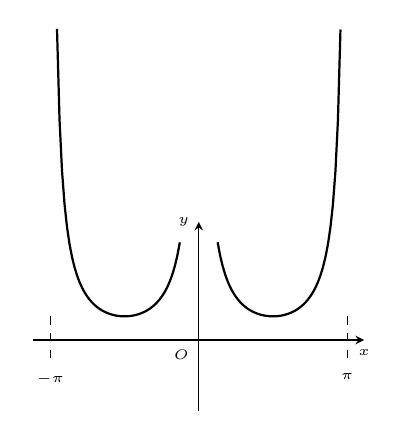
\begin{tikzpicture}[scale=0.6, >=stealth, baseline=(current bounding box.center)]
      \draw[->] (-3.5,0) -- (3.5,0) node[below] {\tiny $x$};
      \draw[->] (0,-1.5) -- (0,2.5) node[left] {\tiny $y$};
      \node[below left] at (0,0) {\tiny $O$};
      \draw[dashed] (3.14,0.5) -- (3.14,-0.5) node[below] {\tiny $\pi$};
      \draw[dashed] (-3.14,0.5) -- (-3.14,-0.5) node[below] {\tiny $-\pi$};
      \draw[thick, domain=0.4:3.0, samples=50] plot (\x, {1/sin(\x r) - 0.5});
      \draw[thick, domain=-3.0:-0.4, samples=50] plot (\x, {1/sin(-\x r) - 0.5});
    \end{tikzpicture}
  }{
    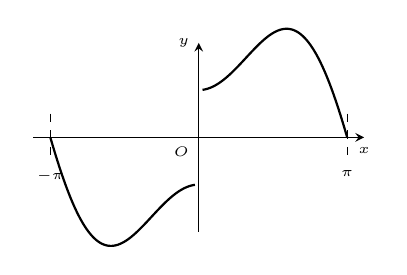
\begin{tikzpicture}[scale=0.6, >=stealth, baseline=(current bounding box.center)]
      \draw[->] (-3.5,0) -- (3.5,0) node[below] {\tiny $x$};
      \draw[->] (0,-2.0) -- (0,2.0) node[left] {\tiny $y$};
      \node[below left] at (0,0) {\tiny $O$};
      \draw[dashed] (3.14,0.5) -- (3.14,-0.5) node[below] {\tiny $\pi$};
      \draw[dashed] (-3.14,0.5) -- (-3.14,-0.5) node[below] {\tiny $-\pi$};
      \draw[thick, domain=0.08:3.14, samples=100] plot (\x, {(\x + 1/\x)*sin(\x r)});
      \draw[thick, domain=-3.14:-0.08, samples=100] plot (\x, {-(-\x + 1/(-\x))*sin(-\x r)});
    \end{tikzpicture}
  }%
}

\newcommand{\qFunctionGraphAnswer}{A}

\newcommand{\qFunctionGraphSolution}{%
  第一步：判断奇偶性。
  定义域为 $[-\pi, 0) \cup (0, \pi]$ 关于原点对称。
  对于定义域内的任意 $x$，有：
  \[ f(-x) = \left(-x + \frac{1}{-x}\right)\sin(-x) = -\left(x + \frac{1}{x}\right)(-\sin x) = \left(x + \frac{1}{x}\right)\sin x = f(x). \]
  因此，函数 $f(x)$ 是偶函数，图象关于 $y$ 轴对称。由此可以排除图 \textbf{D}（D不关于 $y$ 轴对称，故排除）。
  
  第二步：代入特殊值与极限判断。
  当 $x \to 0^+$ 时：
  \[ \lim_{x \to 0^+} f(x) = \lim_{x \to 0^+} \left(x\sin x + \frac{\sin x}{x}\right) = 0 + 1 = 1. \]
  因此，图象在 $x \to 0$ 处极限趋于 $1$。并且当 $x \in (0, \pi)$ 时，有 $x + \dfrac{1}{x} > 0$ 且 $\sin x > 0$，因此 $f(x) > 0$，即图象完全在 $x$ 轴上方。
  在 $x = \pi$ 处，$f(\pi) = 0$。
  
  对比各图象选项：
  图 \textbf{A} 完全符合偶函数、极值极限趋向以及正负性，故选 \textbf{A}。
}

\newcommand{\qFunctionGraphDiagnosis}{%
  学生得分率为 100.0\%。说明学生对函数的奇偶性、函数极值趋势与图象对应关系掌握较为牢固。
}

\newcommand{\qFunctionGraphTeachingNotes}{%
  本题为谭俊文已掌握题目，本次课次计划予以跳过，不占主要讲解时间，直接存档入个人题库。
}


% =====================================================
% 别名兼容：旧课次宏定义
% =====================================================
\newcommand{\qTJWFunctionGraphStem}{\qFunctionGraphStem}
\newcommand{\qTJWFunctionGraphOptions}{\qFunctionGraphOptions}
\newcommand{\qTJWFunctionGraphAnswer}{\qFunctionGraphAnswer}
\newcommand{\qTJWFunctionGraphSolution}{\qFunctionGraphSolution}
\newcommand{\qTJWFunctionGraphDiagnosis}{\qFunctionGraphDiagnosis}
\newcommand{\qTJWFunctionGraphTeachingNotes}{\qFunctionGraphTeachingNotes}
